
\section{Turn Indicator}
\label{sec:turn}

\subsection{Example Description}
\label{sec:turn_desc}

The turn indicator model discussed here is an adaption of a model originally
designed with an industrial partner from the automotive domain\footnote{The
  detailed model is described in~\cite{Peleska&11}.}. The model specifies the
behaviour of a turn indication controller, which essentially supports left and
right flashing as well as emergency flashing. The functionality is modelled
using three inputs (the voltage, the control lever and the emergency flash
button) and two outputs (the states of the left and right turn indication
lights, respectively).
The model can then be used to automatically generate
test cases for a system that shall implement the specified behaviour.
In addition, desired safety properties of the system can also be verified using
model checking.
Both these activities are performed using the RT-Tester Model-Based Test
Case Generator (RTT-MBT) \cite{VSI-mbt-man} and are described in more detail
in Deliverable D5.3a~\cite{INTOCPSD5.3a} and Deliverable D5.3c~\cite{INTOCPSD5.3c}, respectively.

A key feature of this example is that it combines several features which are
important for effective modelling of system specifications using SysML state
charts: It uses variables of different types (voltage is real-valued, the
other ones are integral), it uses hierarchical state machines and concurrent
components.

\subsection{Usage}
\label{sec:turnindicator_usage}

The example is available at \url{https://github.com/into-cps/example_turn_indication}
and can be downloaded as an example project directly from within the
INTO-CPS application. After that, the example can be used for test automation
and model checking activities.

In addition the \emph{VSI tools} release bundle installs a pre-configured RT-Tester project
in the directory \path{C:\Users\<USER>\RTT-Prj\turn-ind\}. The sub-folder \path{sut\}
contains a C~implementation of the system under test. The associated FMU
\path{RTT\_TestProcedures\SUT\TurnIndicationController_sut.fmu} can be run in co-simulated
test run against a generated test driver.


\subsection{SysML}
The model has been developed in Modelio by means of hierarchic parallel state-charts.
Furthermore, architecture diagrams are used to structure components and
ports, and connections are used to express data flow between parallel components.

Figure~\ref{figure:turnindicator:toplevel-achitecture} depicts the structure of
the overall \texttt{System}  which is decomposed in a
\texttt{SystemUnderTest} and a \texttt{TestEnvironment} component.
\begin{figure}[hpt!]
\centerline{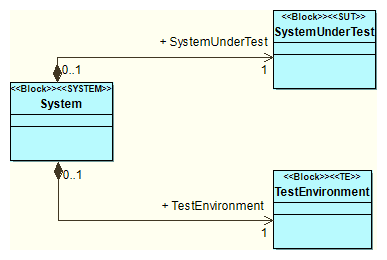
\includegraphics[scale=0.5]{turnindicator/VSI-modelio_turn_indication_small_toplevel_architecture_diagram}}
\caption{Top-level architecture diagram of the turn indicator model.}
\label{figure:turnindicator:toplevel-achitecture}
\end{figure}
The \texttt{SystemUnderTest} encompasses the desired behaviour of the system under test
and has therefore been annotated with the \emph{SUT} stereotype.
The \texttt{TestEnvironment} represents the operational environment to the system under test
and is annotated with the \emph{TE} stereotype.

The system under test receives inputs from the environment and provides outputs.
For both of these, data flow interfaces specify the involved variables
and have been associated with the stereotypes \emph{SUT2TE} and \emph{TE2SUT},
respectively.
The system under test receives the following inputs from the environment:
\begin{itemize}
    \item \texttt{TurnIndLvr}: The position of the turn indicator lever, which can either be
      neutral, left flashing, or right flashing.
    \item \texttt{EmerSwitch}: The on/off status of the emergency flashing switch.
    \item \texttt{voltage}: The voltage of the car's battery.
\end{itemize}
The \texttt{SystemUnderTest} produces the following observable outputs:
\begin{itemize}
    \item \texttt{LampsLeft}: The of/off status of the indication lights on the left side.
    \item \texttt{LampsRight}: The of/off status of the indication lights on the right side.
\end{itemize}
The connection diagram in Figure~\ref{figure:turnindicator:toplevel-connections} connects
the system under test with the test environment using the described interfaces.
\begin{figure}[hpt!]
    \centerline{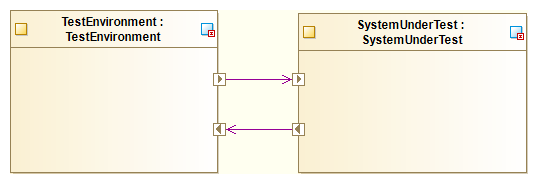
\includegraphics[scale=0.5]{turnindicator/VSI-modelio_turn_indication_small_toplevel_connection_diagram}}
    \caption{Top-level connection diagram of the turn indicator model.}
    \label{figure:turnindicator:toplevel-connections}
\end{figure}

Note, that the correct stereotype annotations of the components are
important for test case generation using RTT-MBT.

In this example, the {\tt TestEnvironment} does not constrain the input
variables in any way (RTT-MBT automatically ensures that the values assigned
during test case generation are within the specified range). The relevant
logic is thus implemented in {\tt SystemUnderTest}, which is divided into two
hierarchical state charts called {\tt FLASH\_CTRL} and {\tt OUTPUT\_CTRL}
as expressed by the class diagram in Figure~\ref{figure:turnindicator:sut-architecture}.
\begin{figure}[hpt!]
    \centerline{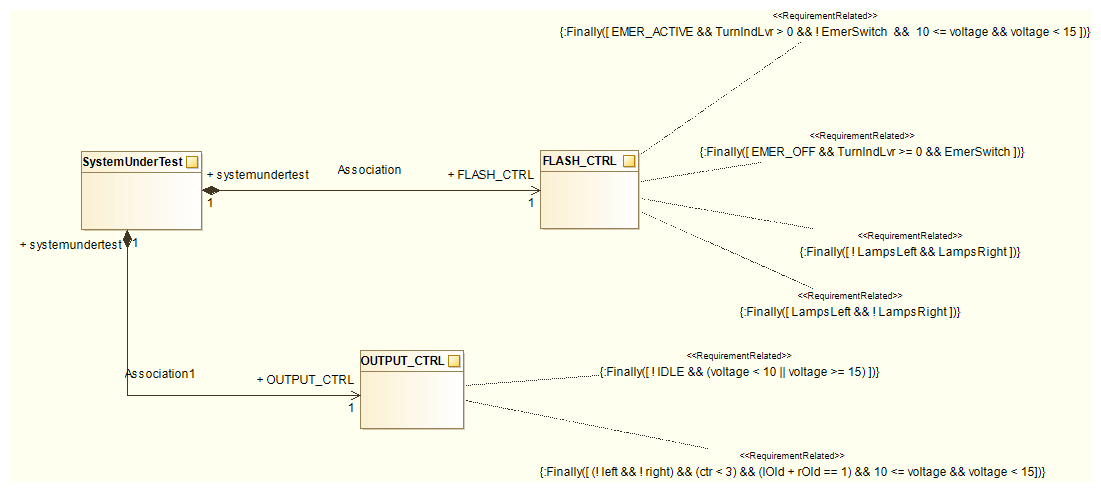
\includegraphics[scale=0.4]{turnindicator/VSI-modelio_turn_indication_small_sut_architecture_diagram}}
    \caption{System under test architecture diagram of the turn indicator model.}
    \label{figure:turnindicator:sut-architecture}
\end{figure}
The component {\tt FLASH\_CTRL} is responsible for deciding whether the left or the
right side has to flash depending on the turn-indicator lever and the emergency switch.
This general decision for the two sides is fed into the {\tt OUTPUT\_CTRL}
which is responsible for periodically turning the lights on and off.
This data flow between the two components is expressed by the connection diagram in
Figure~\ref{figure:turnindicator:sut-connections}.
\begin{figure}[hpt!]
    \centerline{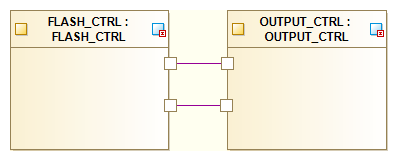
\includegraphics[scale=0.5]{turnindicator/VSI-modelio_turn_indication_small_sut_connection_diagram}}
    \caption{System under test connection diagram of the turn indicator model.}
    \label{figure:turnindicator:sut-connections}
\end{figure}

The {\tt FLASH\_CTRL} state machine in Figure~\ref{figure:vsi-flash-ctrl} controls
the impact of operating the turn indicator
and emergency flashing switch. If the emergency switch is not pressed, the state machine
simply enables flashing on a specific side if the turn indicator lever is in the respective
position.
\begin{figure}[hpt!]
    \centerline{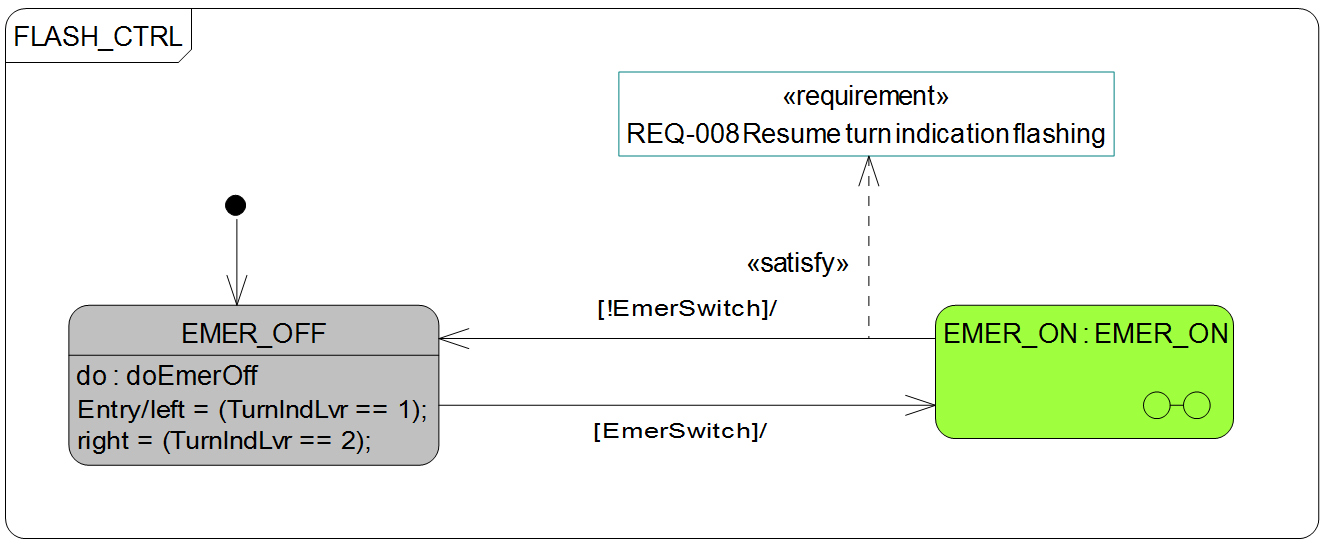
\includegraphics[scale=0.3]{turnindicator/AS_SAMPLE_FLASH_CTRL.png}}
    \caption{The {\tt FLASH\_CTRL} state machine.}
    \label{figure:vsi-flash-ctrl}
\end{figure}
If the emergency switch is pressed, the composite state in Figure~\ref{figure:vsi-emer-on}
decides whether both sides should flash. Observe, that using the turn indicator lever
while the emergency switch is pressed can override emergency flashing.
The lamps resume flashing on both sides when the turn indicator level is returned to
the neutral position.
\begin{figure}[hpt!]
    \centerline{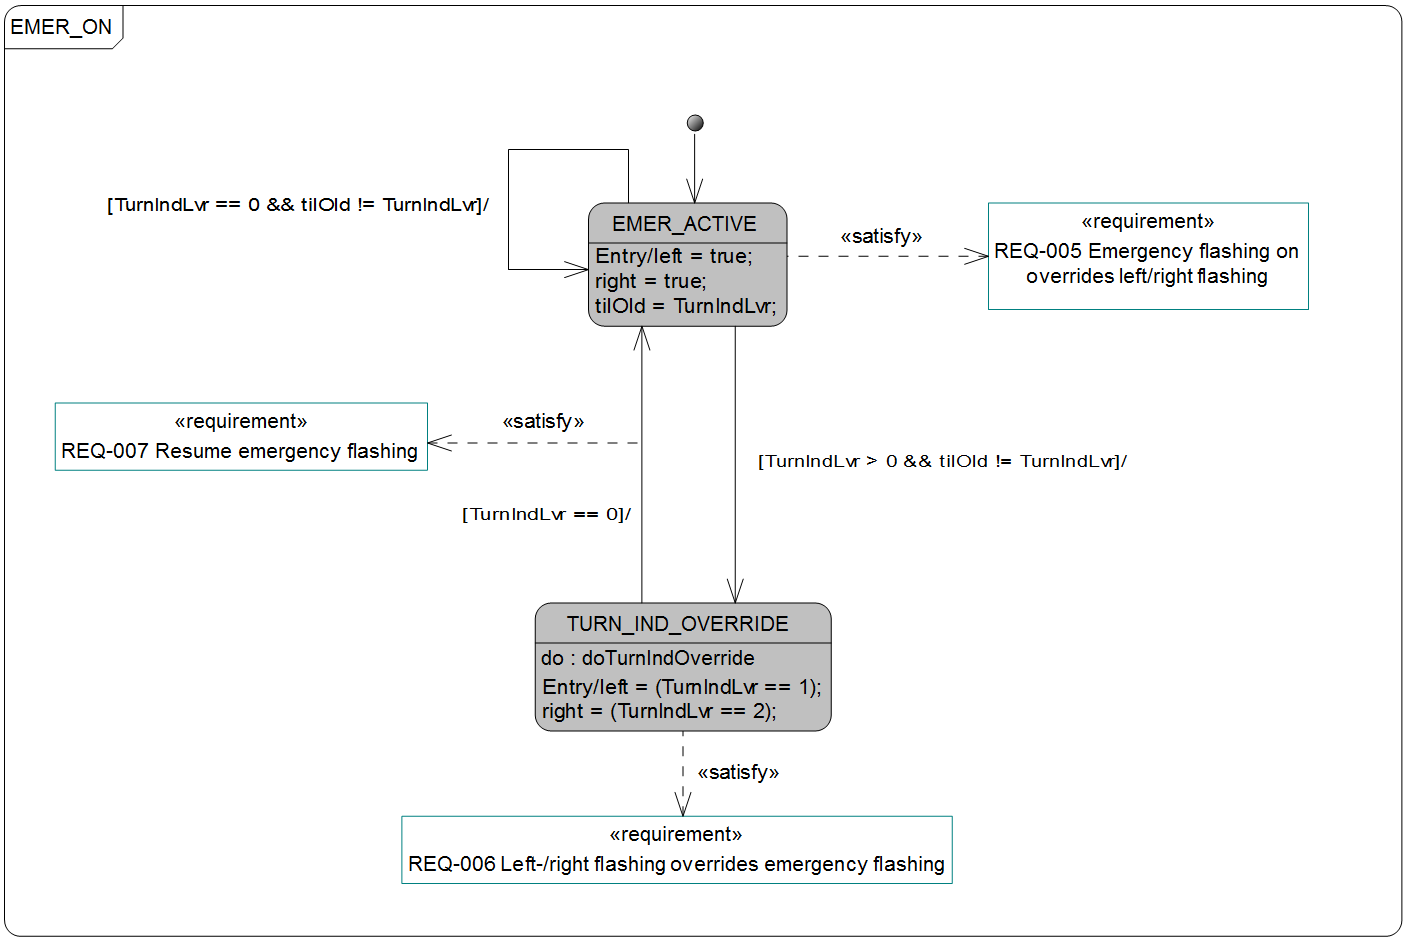
\includegraphics[scale=0.3]{turnindicator/AS_SAMPLE_EMER_ON.png}}
    \caption{The {\tt EMER\_ON} composite state in the {\tt FLASH\_CTRL} state machine.}
    \label{figure:vsi-emer-on}
\end{figure}

{\tt OUTPUT\_CTRL} depicted in Figure~\ref{figure:vsi-output-ctrl} implements two
modes for setting the outputs. It can be in either idle or flashing mode, 
where the flashing mode itself is implemented as composite state that can
switch from off to on and vice versa. It does so in a regular interval if
the system has enough power and a lever or the emergency button has been used.
The state machine also implements a counter that ensures that left or right flashing
is still flashing for three times if the turn indicator level is only operated for a short duration.
\begin{figure}[hpt!]
    \centerline{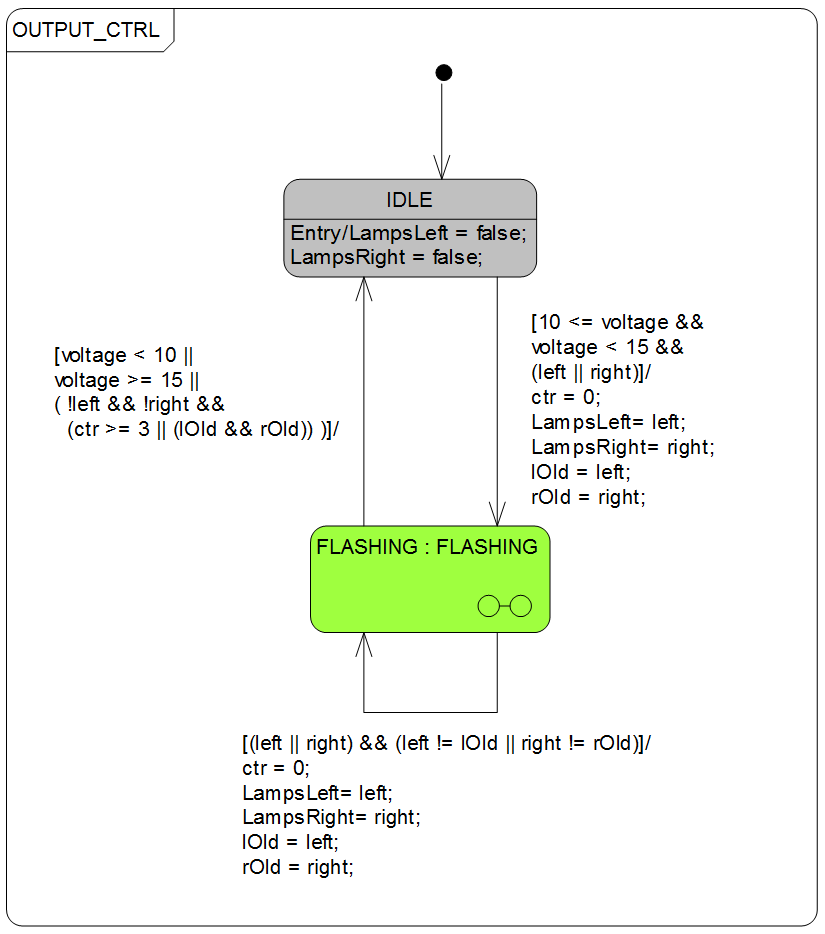
\includegraphics[scale=0.3]{turnindicator/AS_SAMPLE_OUTPUT_CTRL.png}}
    \caption{The {\tt OUTPUT\_CTRL} state machine.}
    \label{figure:vsi-output-ctrl}
\end{figure}

Observe that certain states and transitions in the model have been
annotated with requirements. For example, the transition from state ${\tt
TURN\_IND\_OVERRIDE} \to {\tt EMER\_ACTIVE}$ in
Figure~\ref{figure:vsi-emer-on} has been linked to requirement {\sf REQ-007}
via a \emph{satisfy relation}. Likewise, state {\tt TURN\_IND\_OVERRIDE} has
been linked to requirement {\sf REQ-006}.
Linking requirements in that way specifies that the associated structural elements
of the model help to realise the given requirement.

Furthermore, some requirements are attached to classes in conjunction with an LTL formula
as can be seen in Figure~\ref{figure:turnindicator:sut-architecture}.
The LTL formula specifies an abstract execution trace that could serve as a witness
to demonstrate that the requirement is fulfilled by an implementation.

\subsection{Analyses and Experiments}

\subsubsection{Test Automation and Model Checking}
As mentioned earlier, this pilot can be used to automatically generate
test cases for a system that shall implement the specified behaviour.
In addition, desired safety properties of the system can also be verified using
model checking.
Both these activities are performed using the RT-Tester Model-Based Test
Case Generator (RTT-MBT) and are described in more detail
in Deliverable D5.3a~\cite{INTOCPSD5.3a} and Deliverable D5.3c~\cite{INTOCPSD5.3c}, respectively.
